\chapter{Le stage}
\label{chap:lestage}

\section{Présentation du stage}




\subsection{Présentation}

Le stage pour lequel j'ai postulé consiste au développement de l'application Tastycloud sur tablette. J'ai été recruté pour travailler sur différentes missions et accompagner l'évolution de la plateforme avec la mise en place de nouveaux modules et fonctionnalités. Ces dernières peuvent être de nouveaux projets (et donc commencer quelque chose de zéro) ou bien des missions de maintenance par rapport à des retours clients. J'ai par exemple travaillé sur le tutoriel de l'application depuis zéro et ajouté des options utilisateurs disponibles depuis le back office de l'application pour le restaurateur. Bien sûr tout ceci sera détaillé dans les missions de stages.\\

Aujourd'hui la société a de plus en plus de clients et donc de plus en plus de demandes, de maintenance et de suivi clients. Tout ceci génère donc plus de travail et le besoin d'avoir différentes personnes qui travaillent sur l'application. C'est donc dans ce contexte et avec l'encadrement de mon tuteur que mon stage s'inscrit.\\

\subsection{Étude du poste}

Dans un premier temps, il a été important d'être informé sur le contexte du stage que ce soit d'un point de vue technique ou non. C'est pour cela que j'ai eu des formations par rapport à la solution de l'entreprise, comment la présenter et ce qu'elle contient. J'ai également eu des informations sur les différentes fonctionnalités de l'application sur tablette ou le back office, les avantages pour les clients et les restaurateurs. Il a été important de bien comprendre tous les enjeux de la solution et comment elle fonctionnait pour que mon travail reflète au mieux l'identité de l'entreprise.\\

J'ai également eu la présentation du fonctionnement de l'entreprise côté serveur et application à savoir le serveur test et le serveur de production qui servent comme leur nom l'indique l'un à faire les tests et le deuxième pour les clients. Nous avons à notre disposition un back office test. Les clients ont eux un back office séparé du test (nous parlerons de ça dans la partie suivante).\\

J'ai ensuite eu une formation technique après m'être familiarisé avec le fonctionnement de l'application. On m'a expliqué la structure de l'application et son fonctionnement interne. Que ce soit pour la partie graphique, data ou contrôleur. On m'a, la première semaine du stage expliqué tout ceci en détail et répondu à toutes mes questions. J'ai pu ainsi entreprendre mes premières missions plus sereinement. Il a été décidé que d'abord je ferai des petites missions de maintenance pour me familiariser avec la structure de l'application. Ces premières missions étaient diverses et touchaient surtout la partie graphique et la partie base de données. Il n'y avait donc à ce moment-là pas de réelle modélisation mais juste des petits ajouts ou correction de bug. Cela à bien sûr été bénéfique pour moi avant de me lancer dans de réels projets.

\clearpage

\subsection{Le logiciel sur tablette}

Nous avons, dans la première partie présenté le logiciel sur tablette d'un point de vue client. Nous allons rentrer plus en détail de ce qui était à ma disposition dans la version "dev" de l'application. Il faut savoir que le logiciel a une version "dev" et une version "prod". J'ai travaillé principalement sur la version "dev" et mon tuteur s'occupait de faire les mises en productions. On peut mettre l'application à jour en changeant son code (donc on a affaire à un changement interne du fonctionnement de l'application) ou bien en ajoutant par exemple des vins ou des desserts etc, que l'on peut le faire depuis le back office (que l'on va présenter dans la partie suivante). Nous avons une fonctionnalité sur l'application pour mettre directement à jour les changements faits sur le back office.\\

\begin{figure}[!htb]
  \centering
  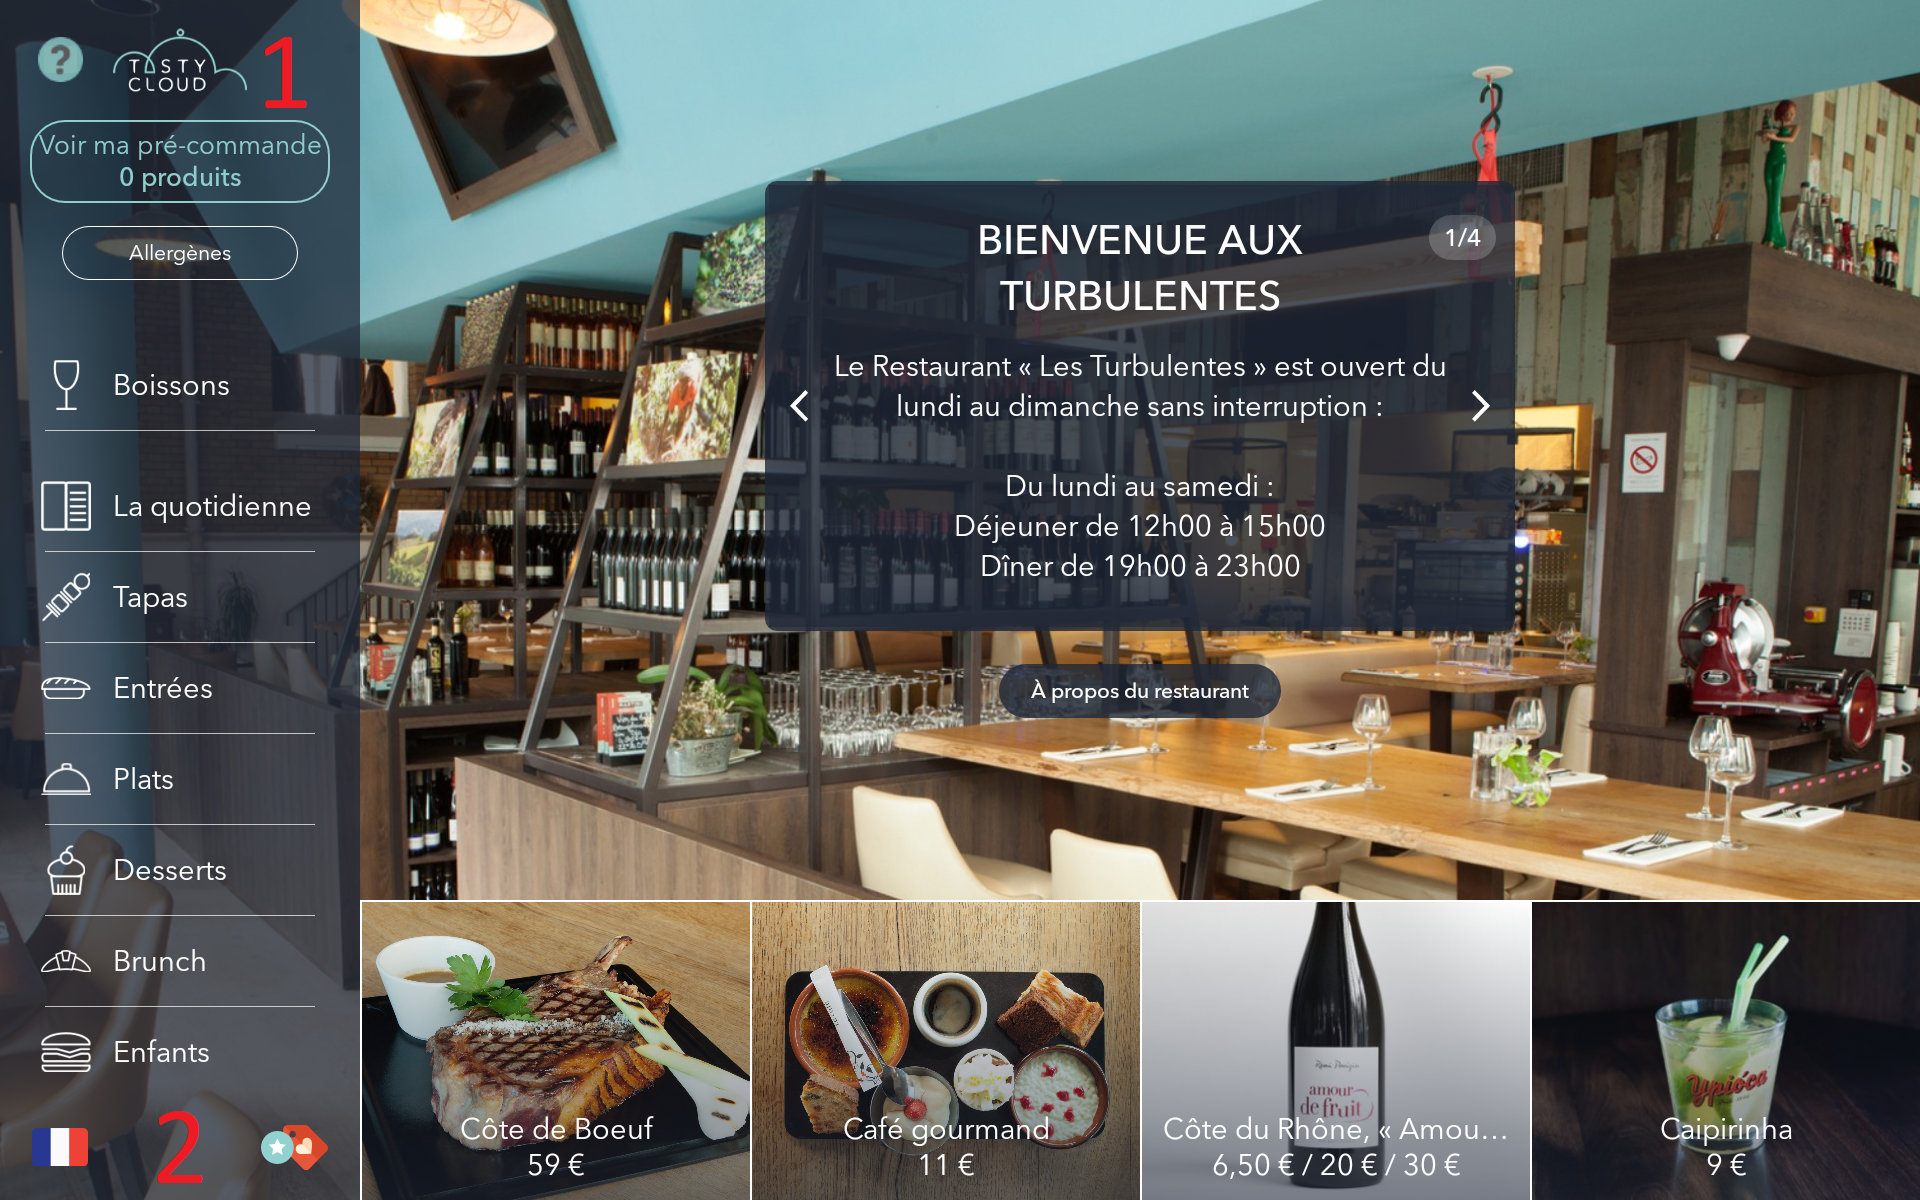
\includegraphics[width=81mm,scale=0.5]{home2_tastycloud.png}
  \caption{Le menu du restaurant "Les Turbulentes"}
  \label{fig:boat1}
\end{figure}

Comme on peut le voir sur la figure ci-dessus, nous avons deux chiffres en rouge. À gauche du 1 c'est le logo de l'application et c'est aussi en faisant ce qu'on appelle un "long click" dessus (donc rester longtemps appuyé sur le logo) qu'on va faire une mise à jour de l'application en synchronisation avec les informations du back office (tout ceci se fait à distance avec le cloud). Pour ce qui est du 2 c'est ici que l'on peut faire un autre "long click" pour accéder à la liste des restaurants sur lesquels on peut naviguer pour faire différents tests (chaque restaurant a ses propres particularités). On peut d'ailleurs vérifier cela avec la présence sur ce restaurant des langues en bas à gauche ce qui n'était pas présent sur le Shogun, le restaurant de l'introduction. On peut voir ci-dessous la page du choix des restaurants, bien sûr ces pages ne sont pas accessibles aux clients du restaurant (voir au restaurateur lui-même).

\begin{figure}[!htb]
  \centering
  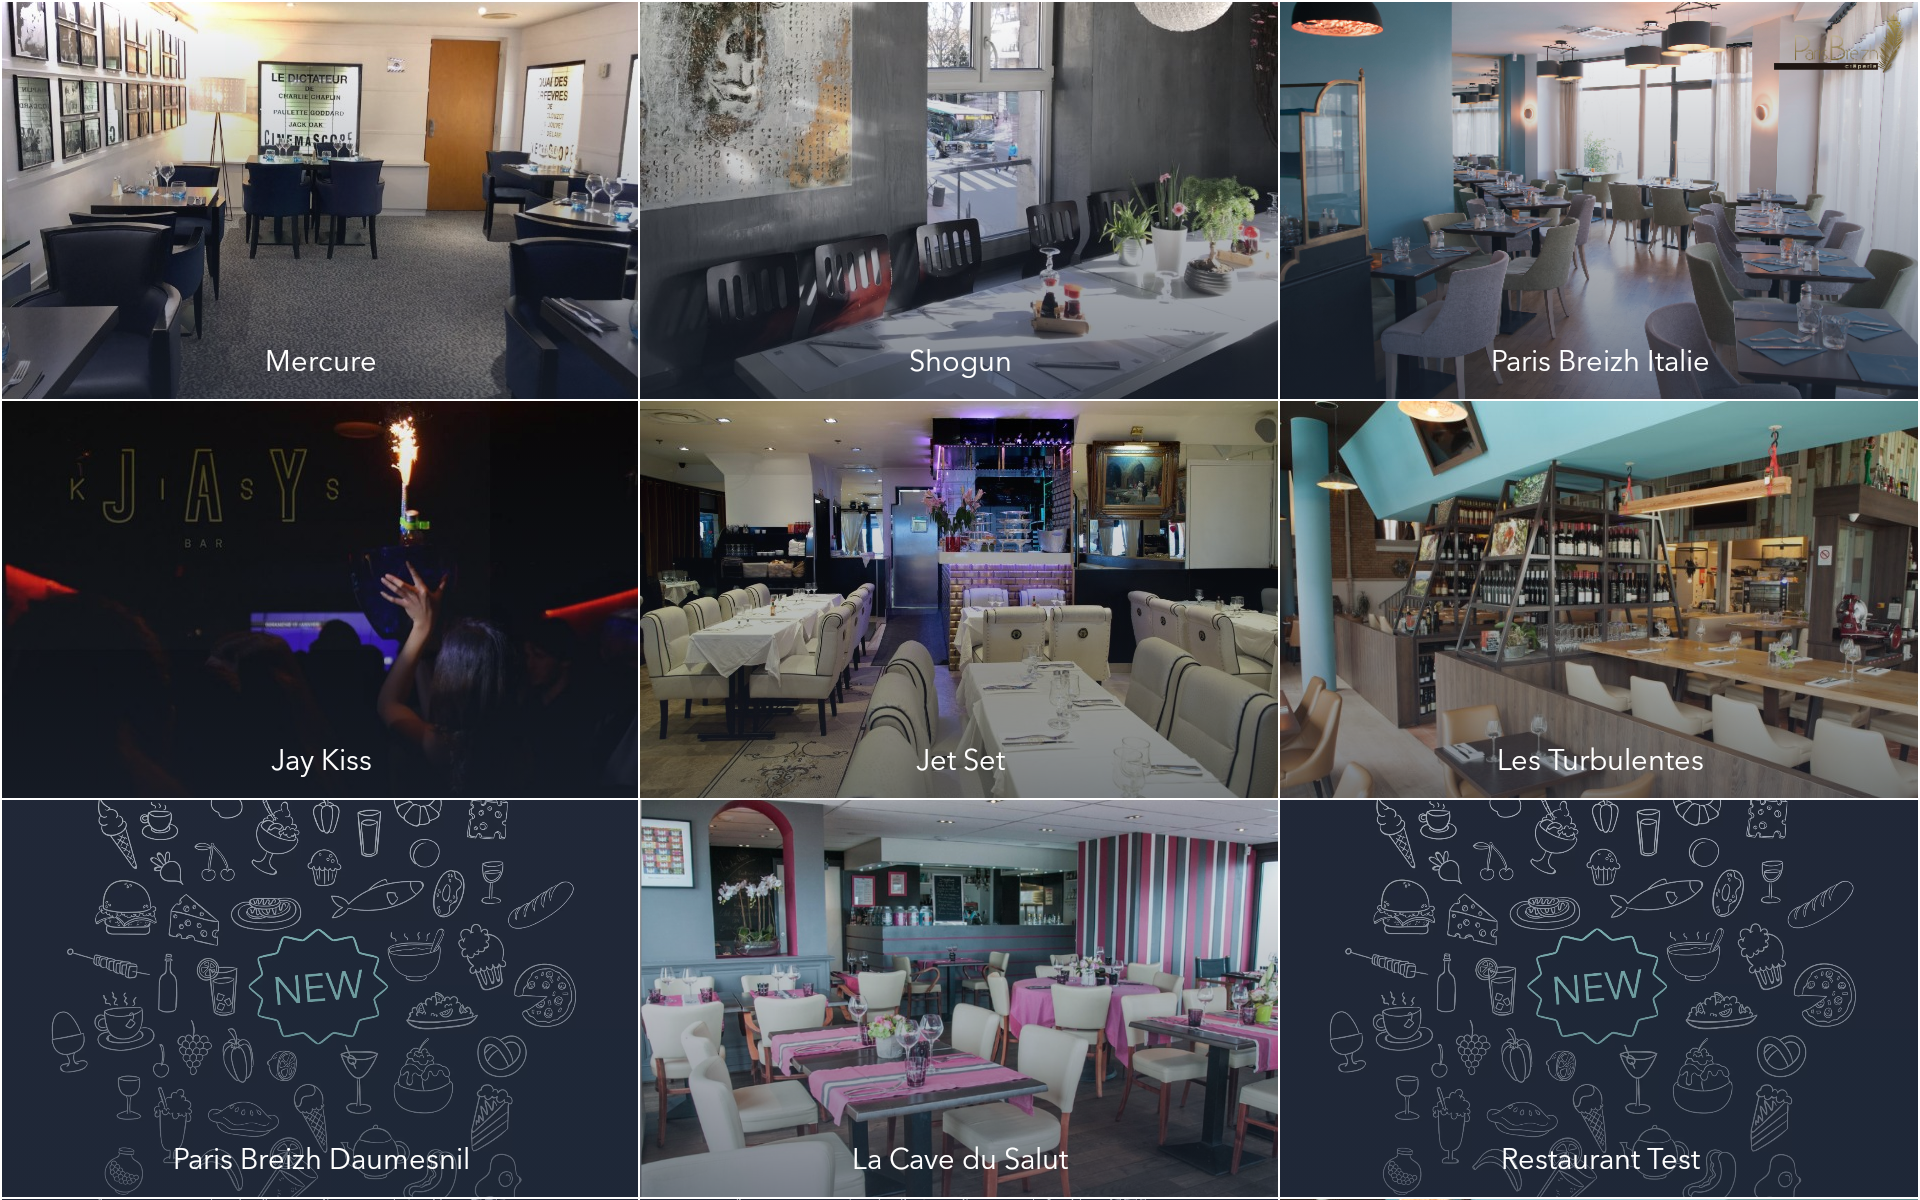
\includegraphics[width=81mm,scale=0.5]{restaurants_tastycloud.png}
  \caption{Page de choix des restaurants}
  \label{fig:boat1}
\end{figure}


\clearpage
\subsection{Le back office}

Le back office est un point essentiel de l'application. C'est ici que sont centralisées toutes les données du restaurant, que ce soit les plats, les boissons, les options, les menus, les descriptions etc... Ce back office est surtout utile pour le restaurateur, c'est avec ce dernier qu'il va pouvoir mettre par exemple à jour sa carte. Comme pour l'application sur tablette, il y a un back office test et prod. Le test est lié à l'application "dev" sur tablette et en toute logique le prod et lié à l'application prod sur tablette. Voyons un aperçu du back office (celui de test) :

\begin{figure}[!htb]
  \centering
  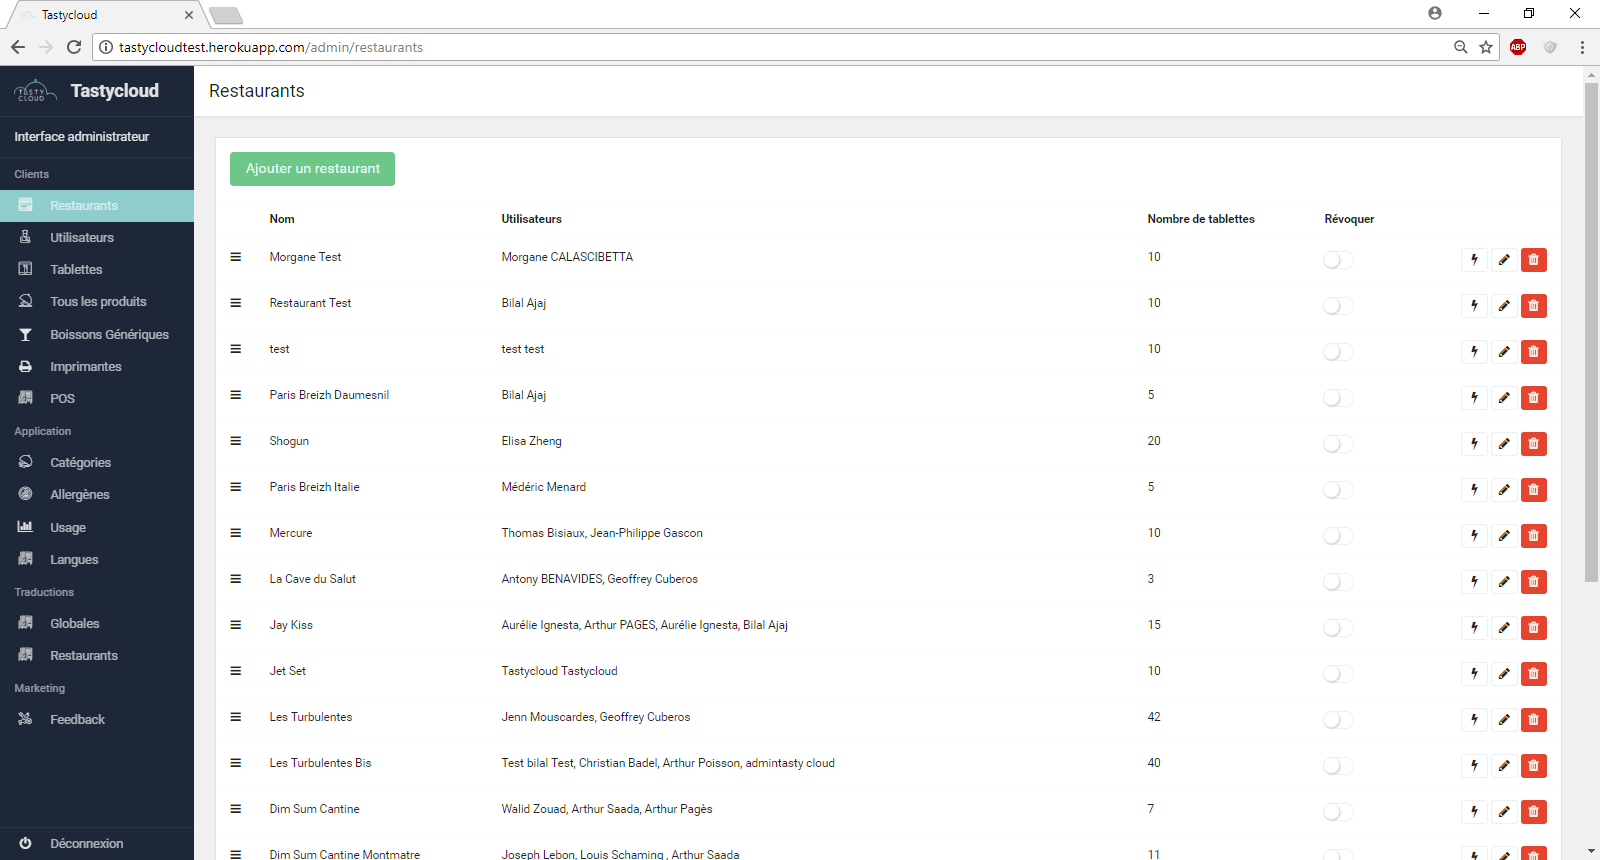
\includegraphics[width=110mm,scale=0.5]{backoffice_tastycloud.png}
  \caption{Back office test}
  \label{fig:boat1}
\end{figure}

Comme nous pouvons le voir sur la figure ci-dessus, le back office contient un menu à gauche et la liste des restaurants dans la fenêtre à droite. C'est sur ce back office que l'on peut par exemple rajouter des tablettes et les affilier à un restaurant. Pour cela on peut cliquer sur l'édition d'un restaurant (bouton à gauche des trois boutons sur la droite d'un restaurant) et par exemple y ajouter de nouvelles tablettes, une nouvelle formule, de nouvelles traductions etc...

\begin{figure}[!htb]
  \centering
  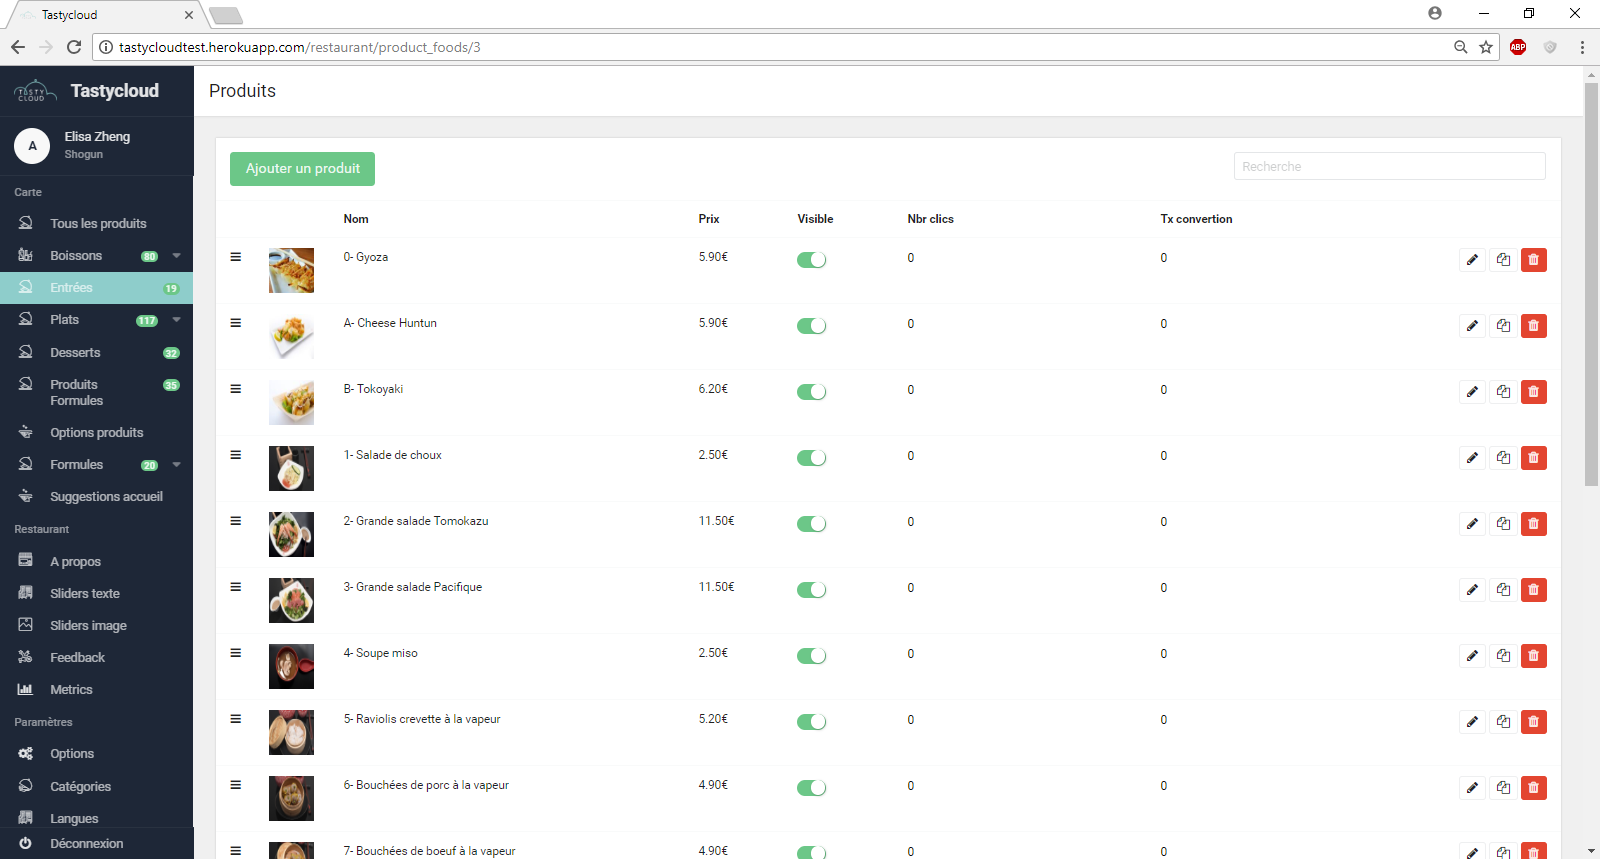
\includegraphics[width=110mm,scale=0.5]{backoffice2_tastycloud.png}
  \caption{Restaurant "Shogun" dans le back office test}
  \label{fig:boat1}
\end{figure}

\section{Technologies et outils utilisés}

\subsection{Android Studio et languages}

L'IDE utilisé pour le développement sur tablette a été Android Studio, nous n'avons pas utilisé d'émulateur puisque les tablettes pour les tests sont fournies. Par rapport au moteur de production (pour builder l'application) nous utilisons Gradle. Les langages utilisés ont principalement été Kotlin et le XML. Kotlin est aujourd'hui un langage supporté officiellement par Android et proche de JAVA. On peut en effet convertir du JAVA en Kotlin (ça ne marche pas tout le temps mais ça existe). Il est intéropérable avec JAVA, qui est le premier langage supporté par Android. Kotlin est un langage récent mais qui propose des avantages pour la sécurité et l'extensibilité du code. Il a en effet des fonctionnalités intéressantes en termes de nullabilité et d'immutabilité. Pour la partie graphique c'est XML qui est utilisé, un langage de balisage qui permet une facilité de lecture et de conception en terme d'arborescence d'éléments. Toutes les vues (éléments qui composent les pages) sont donc définies en XML.\\



\begin{figure}[!htp]
  \centering
  \begin{minipage}[b]{0.2\textwidth}
    
\includegraphics[width=\textwidth]{logo_androidstudio.png}
    \caption{Logo Android}
  \end{minipage}
  \hfill
  \begin{minipage}[b]{0.2\textwidth}
    
\includegraphics[width=\textwidth]{logo_kotlin.png}
    \caption{Logo Kotlin}
  \end{minipage}
  \hfill
  \begin{minipage}[b]{0.2\textwidth}
    
\includegraphics[width=\textwidth]{logo_xml.png}
    \caption{Logo XML}
  \end{minipage}
\end{figure}

\subsection{Les tablettes}

Pour ce qui est des tablettes ce sont des Galaxy Tab A modèle SM-T580. Le logiciel est essentiellement distribué sur ce modèle et donc la taille (10,1 pouces) est unique. Nous n'avons donc pas besoin de prévoir différentes tailles dans le développement de l'application. Ce sont les tablettes fournies aux clients.

\begin{figure}[!htb]
  \centering
  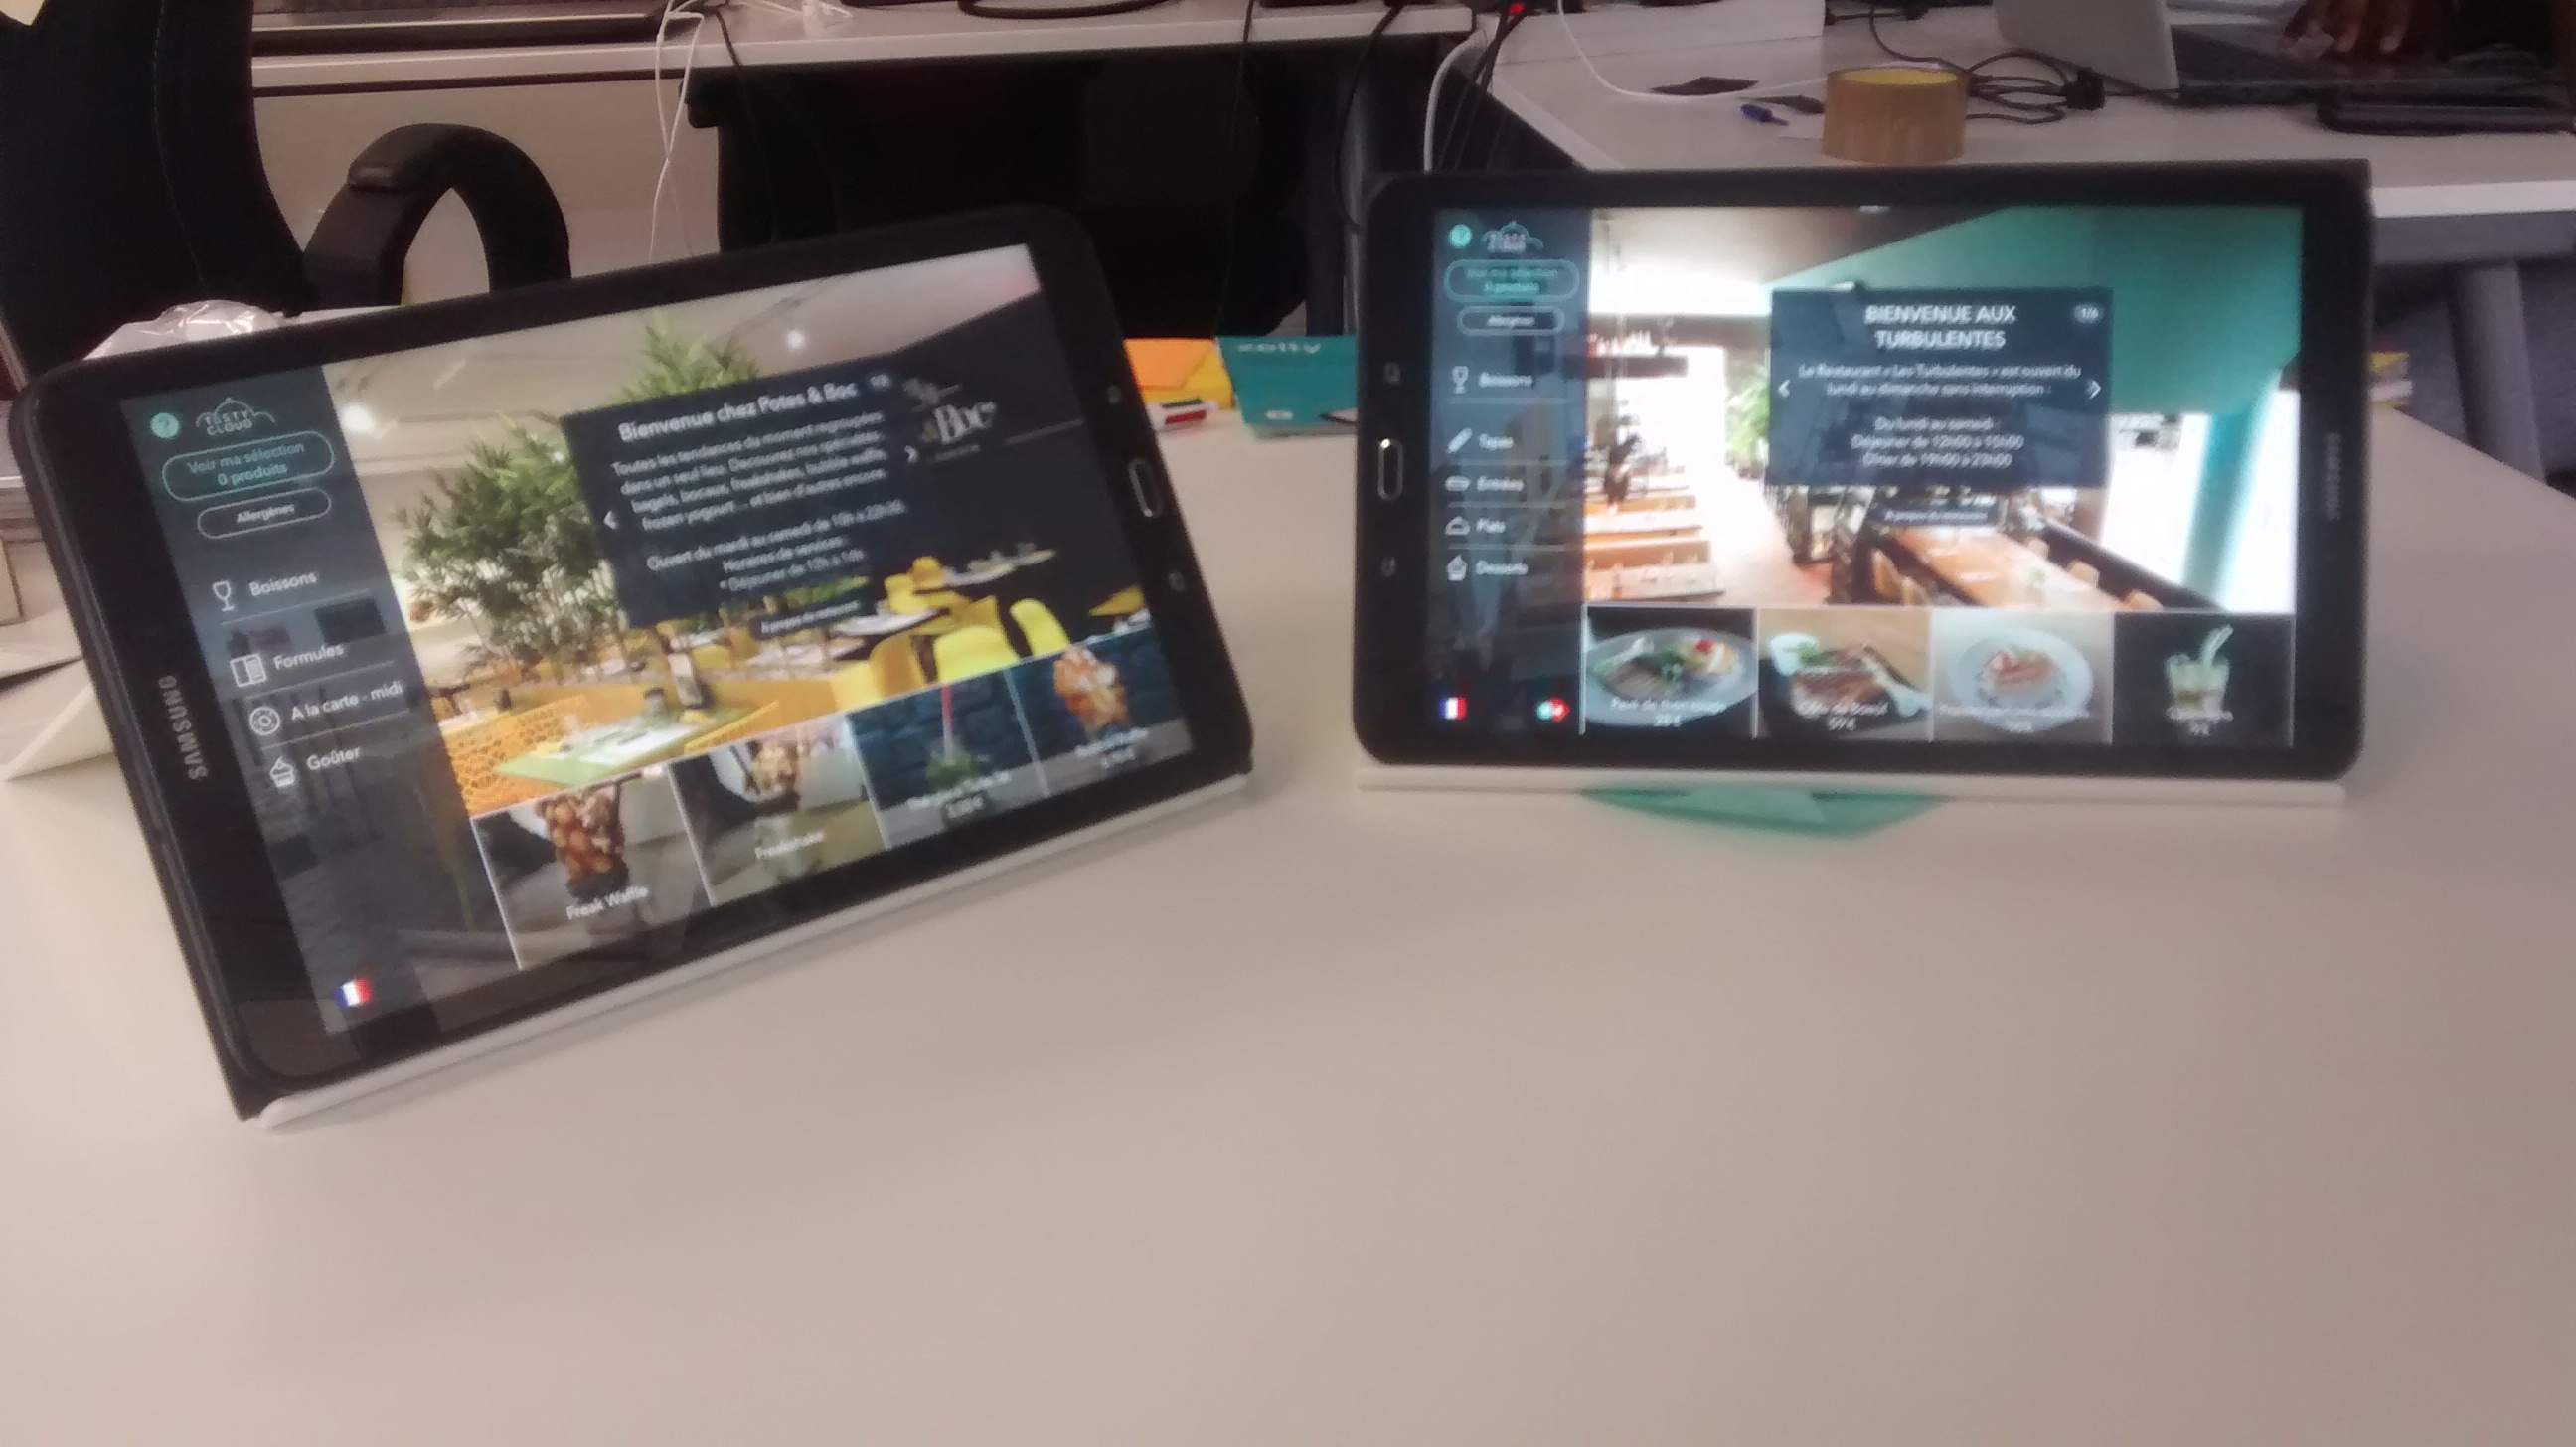
\includegraphics[width=105mm,scale=0.5]{img_tablettes.jpg}
  \caption{Aperçu des tablettes avec l'application}
\end{figure}

\subsection{Git, bit bucket}

Ne travaillant pas seul sur le développement du logiciel et étant amené à travailler en collaboration il a donc été décidé de travailler avec un logiciel de gestion de versions décentralisé tel que git. Ce dernier permet donc à l'équipe de pouvoir échanger des versions du logiciel selon qui travaille sur quoi. C'est ainsi que je peux travailler sur mes propres projets pendant que mon tuteur lui travaille sur autre chose. On met alors en commun ce travail à l'aide de git. Le service web utilisé pour l'hébergement et la visualisation des versions est BitBucket.

\begin{figure}[!htb]
  \centering
  \begin{minipage}[b]{0.25\textwidth}
    
\includegraphics[width=\textwidth]{logo_git.png}
    \caption{Logo git}
  \end{minipage}
  \hfill
  \begin{minipage}[b]{0.3\textwidth}
    
\includegraphics[width=\textwidth]{logo_bitbucket.png}
    \caption{Logo bitbucket}
  \end{minipage}
\end{figure}


\subsection{Outils de communication}

Nous avons utilisé divers outils de communication durant le stage, de manière formelle comme avec des réunions ou des points de parcours, ou de manière organisationnelle avec des logiciels. Les principaux outils logiciels utilisés ont été Basecamp pour la mise en place des tâches et l'affectation de tâches. Basecamp est un outil web de gestion de projet qui permet notamment de me donner des "to-do" qui signifie des objectifs à réaliser dans un temps donné. Chaque tâche peut être plus ou moins complexe et le logiciel permet de communiquer et "taguer" des gens sur cette tâche. C'est un outil pratique car il donne la possibilité de communiquer facilement avec toute l'équipe sur un point donné.

Pour le cas de Basecamp, ce dernier permet de communiquer notamment avec la partie non technique de l'entreprise (par exemple pour communiquer sur des aspects graphiques). Pour l'aspect purement technique nous avons utilisé Slack. Nous avions notamment des channels par rapport à la partie Android et NodeJs.

Enfin dans un souci pratique nous avons également utilisé Whatsapp si nous devions communiquer rapidement et par téléphone lorsque mon tuteur était en déplacement par exemple.

\begin{figure}[!htb]
  \centering
  \begin{minipage}[b]{0.2\textwidth}
    
\includegraphics[width=\textwidth]{logo_basecamp.png}
    \caption{Logo Basecamp}
  \end{minipage}
  \hfill
  \begin{minipage}[b]{0.2\textwidth}
    
\includegraphics[width=\textwidth]{logo_slack.png}
    \caption{Logo Slack}
  \end{minipage}
    \hfill
  \begin{minipage}[b]{0.2\textwidth}
    
\includegraphics[width=\textwidth]{logo_whatsapp.png}
    \caption{Logo Whatsapp}
  \end{minipage}
\end{figure}



%%% Local Variables: 
%%% mode: latex
%%% TeX-master: "isae-report-template"
%%% End: 